\section{すべてをまとめる}

多くの場合、シーケンシャルデータの処理は同じようなパターンで行われます。

\begin{enumerate}
\item  どんな質問をしようとしているのかを把握する。このステップは、問題領域やビジネス領域に位置するため、最も困難な場合が多い。明確な質問があれば、Clojureはあなたが持っているデータを処理して答えを出すためのツールを提供します。それが次の3つのステップです。
\item  データをフィルタリングして、不要な要素を取り除く。
\item 要素を目的の形に変換する。
\item 変換された要素を答えに還元する。
\end{enumerate}


ショッピングカートの例で説明しましょう。オンラインストアでは、カタログ、つまり販売する商品のリストがあります。これらの商品は部門ごとに分けられています。顧客はそれらをカートに入れ、チェックアウトする。このプロセスで、請求記録が作成されます。あなたの顧客は、部門別の売上を要約したレポートを要求しています:すべての決済されたカートについて、部門ごとの総売上はいくらですか?

ドメインモデルは次のとおりです。


\begin{lstlisting}[numbers=none]
(require '[money :refer [make-money +$ *$]])

(defrecord CatalogItem [number dept desc price])
(defrecord Cart        [number customer line-items settled?])
(defrecord LineItem    [quantity catalog-item price])
(defrecord Customer    [cname email membership-number])
\end{lstlisting}

何度もチェックアウトを繰り返すと、カートには\texttt{\#Cart}レコードのベクターが含まれることがあります。


\begin{lstlisting}[numbers=none]
[#Cart{:number 116,
       :customer #Customer{:cname "Danny Tanner",
                           :email "danny@fullhouse.example.com",
                           :membership-number 28374},
       :line-items [
         #LineItem{:quantity 3,
                   :catalog-item #CatalogItem{:number 664,
                                              :dept :clothing,
                                              :desc "polo shirt L",
                                              :amount 2515 :currency :usd},
                   :price #Money{:amount 7545
                                 :currency :usd}
         #LineItem{:quantity 1,
                   :catalog-item #CatalogItem{:number 621,
                                              :dept :clothing,
                                              :desc "khaki pants",
                                              :price #Money{:amount 3500
                                                            :currency
                                                            :usd},
                   :price #Money{:amount 3500
                                 :currency :usd}
                    ],
       :settled? true}, ,,, ]
\end{lstlisting}


これはかなり大きなデータ構造で、次の図のようなクラス図で理解するのが分かりやすいかもしれません。

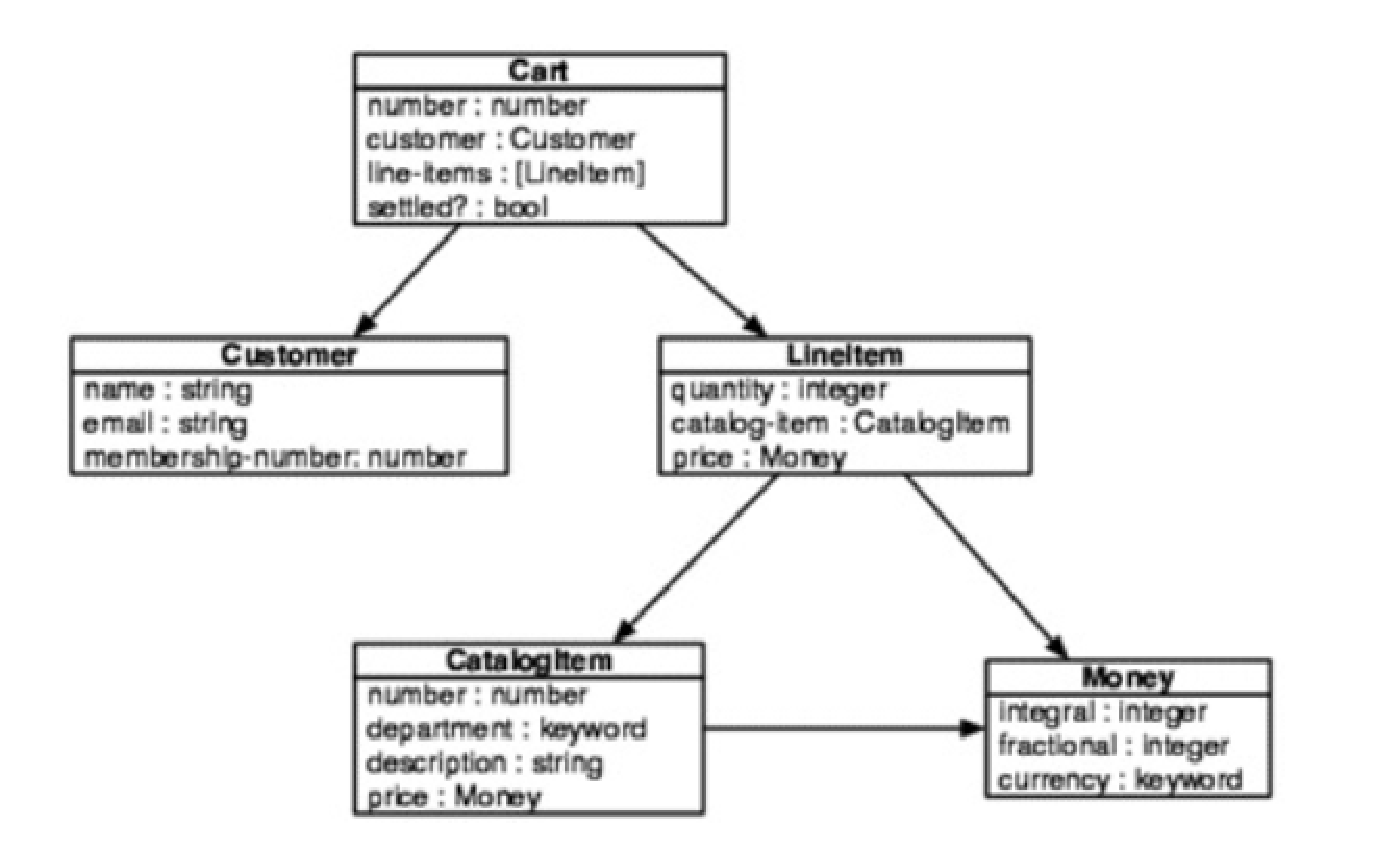
\includegraphics[width=12cm]{fig_03_001.eps}

